%
% Assignment Template
% Last modified 9/11/2024 by Ziyong Wang

\documentclass[11pt]{article}
\usepackage[left=0.7in,right=0.7in,top=1in,bottom=0.7in]{geometry}
\usepackage{fancyhdr} % for header
\usepackage{graphicx} % for figures
\usepackage{amsmath}  % for extended math markup
\usepackage{amssymb}
\usepackage{inconsolata}
\usepackage{enumitem}
\usepackage{float}
\usepackage[bookmarks=false]{hyperref} % for URL embedding
\usepackage[noend]{algpseudocode} % for pseudocode
\usepackage[plain]{algorithm} % float environment for algorithms
\usepackage{array}
\usepackage{booktabs}

%%%%%%%%%%%%%%%%%%%%%%%%%%%%%%%%%%%%%%%%%%%%%%%%%%%%%%%%%%%%%%%%%%%%%%

\newcommand{\Course}{FIN 550E}
\newcommand{\GroupNumber}{27}
\newcommand{\ProjectNumber}{1}

%%%%%%%%%%%%%%%%%%%%%%%%%%%%%%%%%%%%%%%%%%%%%%%%%%%%%%%%%%%%%%%%%%%%%%%%

% create header and footer for every page
\pagestyle{fancy}
\fancyhf{}
\lhead{\textbf{\Course}}
\chead{\textbf{Group \GroupNumber}}
\rhead{\textbf{Empirical Project \ProjectNumber}}
\cfoot{\thepage}

% preferred pseudocode style
\algrenewcommand{\algorithmicprocedure}{}
\algrenewcommand{\algorithmicthen}{}

% ``do { ... } while (cond)''
\algdef{SE}[DOWHILE]{Do}{doWhile}{\algorithmicdo}[1]{\algorithmicwhile\ #1}%

% ``for (x in y ... z)''
\newcommand{\ForRange}[3]{\For{#1 \textbf{in} #2 \ \ldots \ #3}}

% these are common math formatting commands that aren't defined by default
\newcommand{\union}{\cup}
\newcommand{\isect}{\cap}
\newcommand{\ceil}[1]{\ensuremath \left\lceil #1 \right\rceil}
\newcommand{\floor}[1]{\ensuremath \left\lfloor #1 \right\rfloor}

%%%%%%%%%%%%%%%%%%%%%%%%%%%%%%%%%%%%%%%%%%%%%%%%%%%%%%%%%%%%%%%%%%%%%%

\begin{document}

% text goes here!

\section{Part 1: data preparation}

\begin{enumerate}
\renewcommand{\labelenumi}{(\theenumi)}
    \item \, \\
    \begin{table}[H]
        \centering
        \begin{tabular}{lccc}
        \hline
         & \textbf{s} & \textbf{netwin1} & \textbf{netwin2} \\
        \hline
        \textbf{mean} & -0.034295 & 0.000546 & 0.008731 \\
        \textbf{std} & 6.910801 & 0.085145 & 0.340307 \\
        \textbf{min} & -1790.209 & -0.890778 & -1.071007 \\
        \textbf{10th percentile} & -0.005455 & -0.083904 & -0.316339 \\
        \textbf{25th percentile} & -0.000437 & -0.033229 & -0.152914 \\
        \textbf{median} & 0.000331 & 0.000182 & -0.012081 \\
        \textbf{75th percentile} & 0.001659 & 0.034908 & 0.128584 \\
        \textbf{90th percentile} & 0.004961 & 0.084568 & 0.313767 \\
        \textbf{max} & 7.432727 & 1.588795 & 22.972540 \\
        \hline
        \end{tabular}
        \caption{Summary Statistics for Earnings Surprises (s), Market-Adjusted Returns for Windows [0,1] (\texttt{netwin1}) and [3,75] (\texttt{netwin2})}
    \end{table}

    \item All 3 data series have significant outliers. The earnings surprise data is the most affected while \texttt{netwin1} 
    seems to be the least affected. This can be infered from the Kurtosis number and by comparing the standard 
    deviation and sample variance to the mean.
    The presence of outliers can increase the likelihood of both Type I errors (false positives) 
    and Type II errors (false negatives) by affecting test statistics.
    The largest 339th number and the smallest 339th are the winsorization values at 0.05\% and 99.5\%. 
    This is the same as the winsorization values for \texttt{sw}, \texttt{netwin1w}, \texttt{netwin2w}.
    
    \begin{table}[H]
        \centering
        \begin{tabular}{>{\raggedright\arraybackslash}p{4cm} c c c}
        \toprule
         & \textbf{s} & \textbf{netwin1} & \textbf{netwin2} \\
        \midrule
        Mean                   & (0.03)        & 0.00          & 0.01          \\
        Standard Error         & 0.03          & 0.00          & 0.00          \\
        Median                 & 0.00          & 0.00          & (0.01)        \\
        Mode                   & -             & (0.01)        & (0.10)        \\
        Standard Deviation     & 6.91          & 0.09          & 0.34          \\
        Sample Variance        & 47.76         & 0.01          & 0.12          \\
        Kurtosis               & 66,564.25     & 11.71         & 405.61        \\
        Skewness               & (257.06)      & 0.30          & 9.04          \\
        Range                  & 1,797.64      & 2.48          & 24.04         \\
        Minimum                & (1,790.21)    & (0.89)        & (1.07)        \\
        Maximum                & 7.43          & 1.59          & 22.97         \\
        Sum                    & (2,320.06)    & 36.96         & 590.65        \\
        Count                  & 67,649        & 67,649        & 67,649        \\
        Largest (339)          & 0.05818       & 0.31124       & 5.70          \\
        Smallest (339)         & (0.16225)     & (0.31321)     & (0.96)        \\
        Confidence Level (95.0\%) & 0.05208   & 0.00064       & 0.00          \\
        \bottomrule
        \end{tabular}
        \caption{Summary Statistics}
    \end{table}

\end{enumerate}

\section{Part 2: short-run response}

\begin{enumerate}
\setcounter{enumi}{2}
\renewcommand{\labelenumi}{(\theenumi)}
    \item \, \\
    
    \begin{figure}[H] 
        \centering
        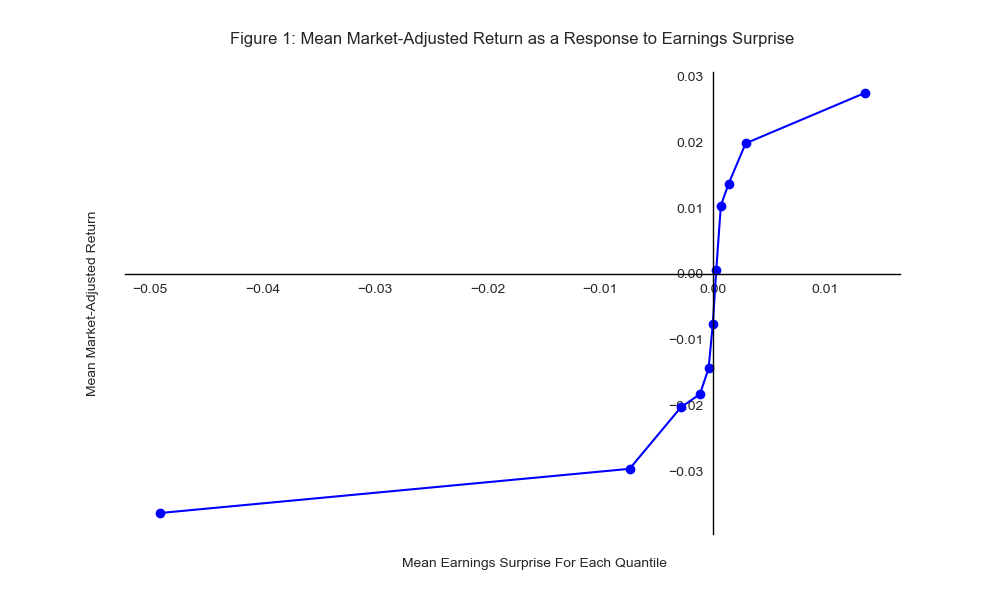
\includegraphics[width=.8\textwidth]{fig1.png}
    \end{figure}

    \begin{figure}[H] 
        \centering
        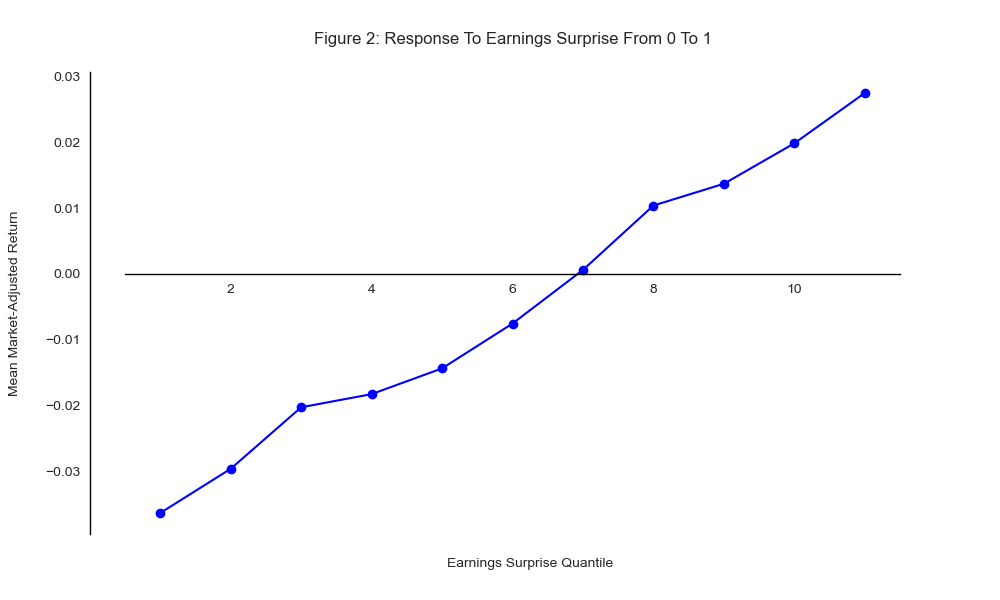
\includegraphics[width=.8\textwidth]{fig2.png}
    \end{figure}
    
    \item
    
    \item

\end{enumerate}

\section{Part 3: Post-earnings announcement drift}

\begin{enumerate}
\setcounter{enumi}{5}
\renewcommand{\labelenumi}{(\theenumi)}
    \item \, \\
    \begin{figure}[H] 
        \centering
        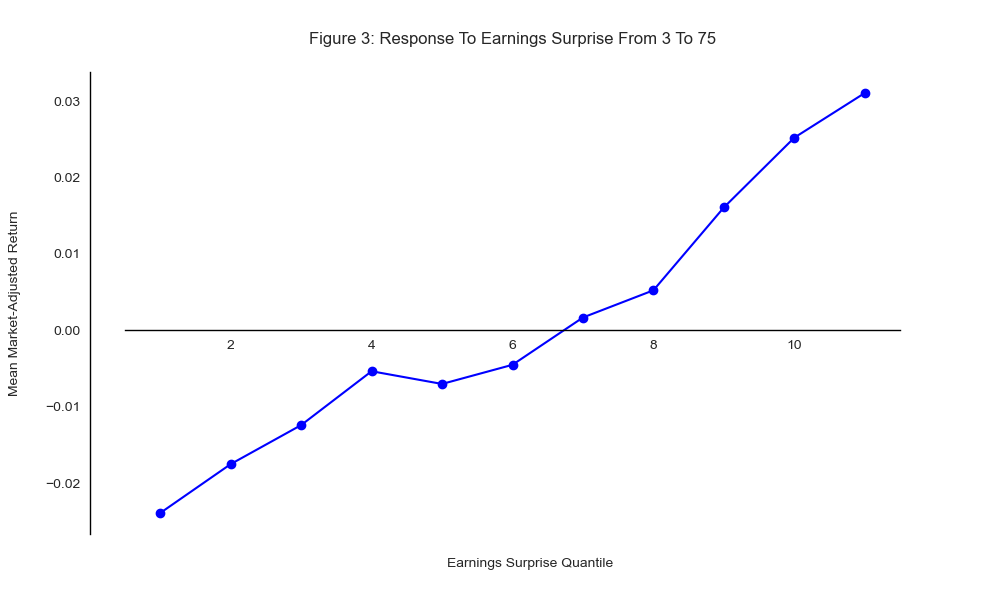
\includegraphics[width=.8\textwidth]{fig3.png}
    \end{figure}
    
    \item The efficient market hypothesis (EMH) says that stock prices should immediately reflect all known information. 
    This means that all responses to unexpected earnings should happen right now, and there shouldn't be a pattern in 
    returns afterward. After the earnings report, we wouldn't expect any systematic post-announcement shift in 
    the [3,75] window, no matter how big the earnings surprise was. However, the plot shows that earnings surprise 
    quantiles (\texttt{sw\_quantiles}) and post-announcement drift (\texttt{netwin2w}) are related. Higher surprises 
    in earnings are related to higher average returns in the [3,75] window. It seems that the market doesn’t fully get 
    information from earnings reports immediately, so prices change slowly. This result goes against the efficient 
    market theory, showing that markets may take a while to fully get information about earnings.
    
    \item 


\end{enumerate}

\section{Part 4: Inattention and distractions}

\begin{enumerate}
\setcounter{enumi}{8}
\renewcommand{\labelenumi}{(\theenumi)}
    \item 

\end{enumerate}

\section{Part 5: Open-ended}

\begin{enumerate}
\setcounter{enumi}{9}
\renewcommand{\labelenumi}{(\theenumi)}
    \item 

    \item

\end{enumerate}

\section{Appendix}
\begin{figure}[H] 
    \centering
    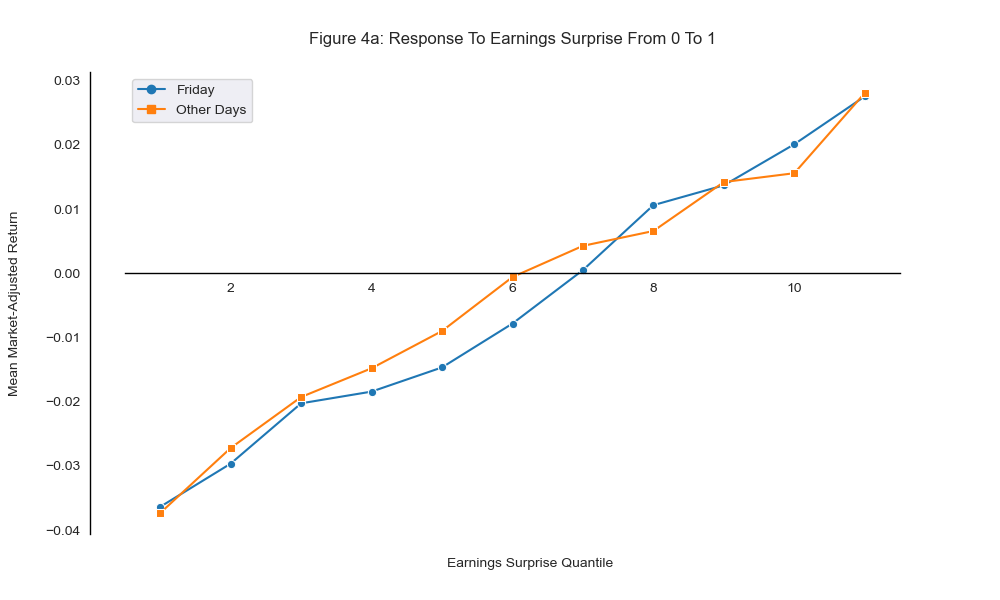
\includegraphics[width=.8\textwidth]{fig4a.png}
\end{figure}

\begin{figure}[H] 
    \centering
    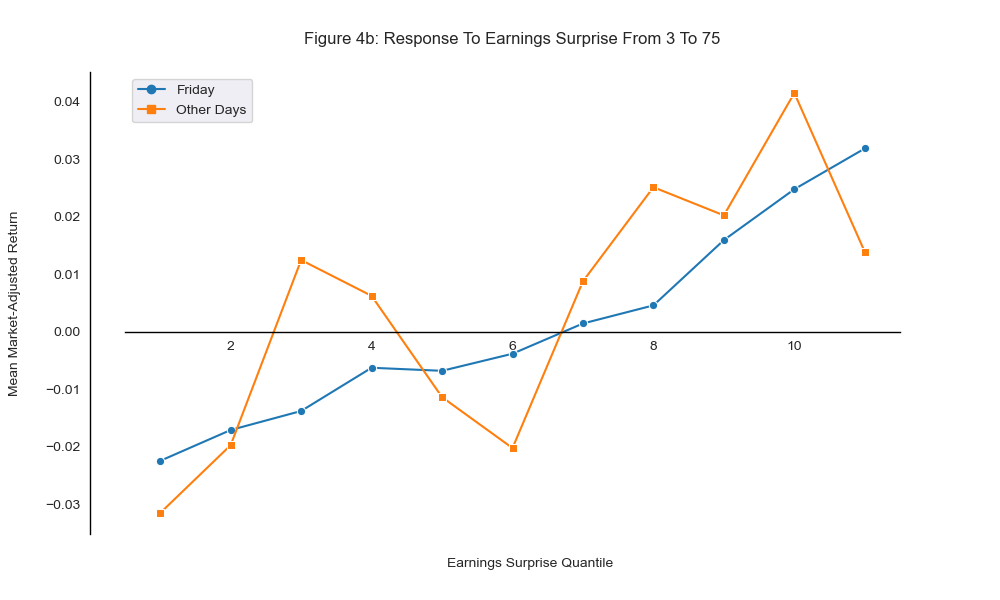
\includegraphics[width=.8\textwidth]{fig4b.png}
\end{figure}

\begin{figure}[H] 
    \centering
    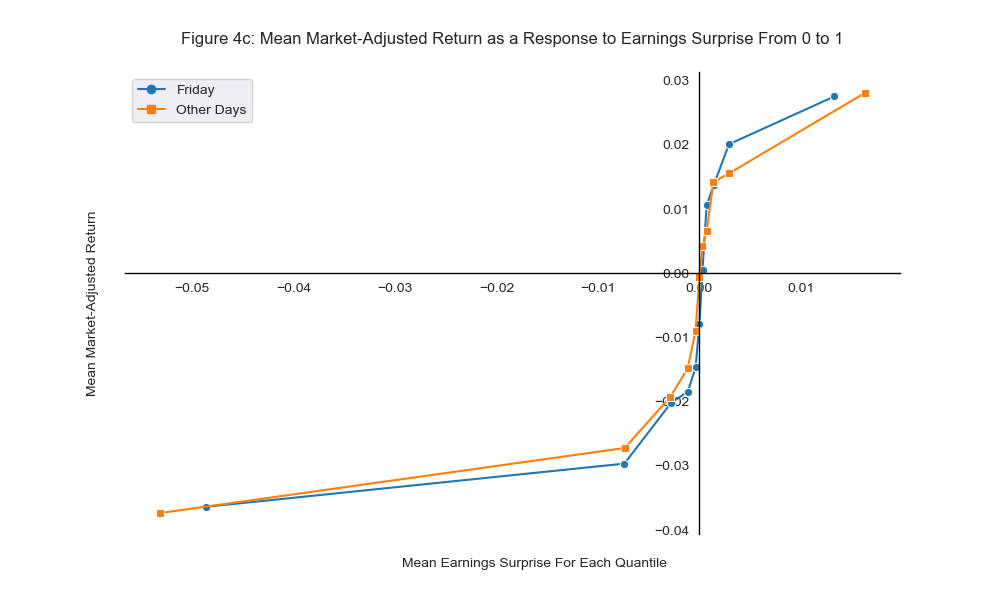
\includegraphics[width=.8\textwidth]{fig4c.png}
\end{figure}

\begin{figure}[H] 
    \centering
    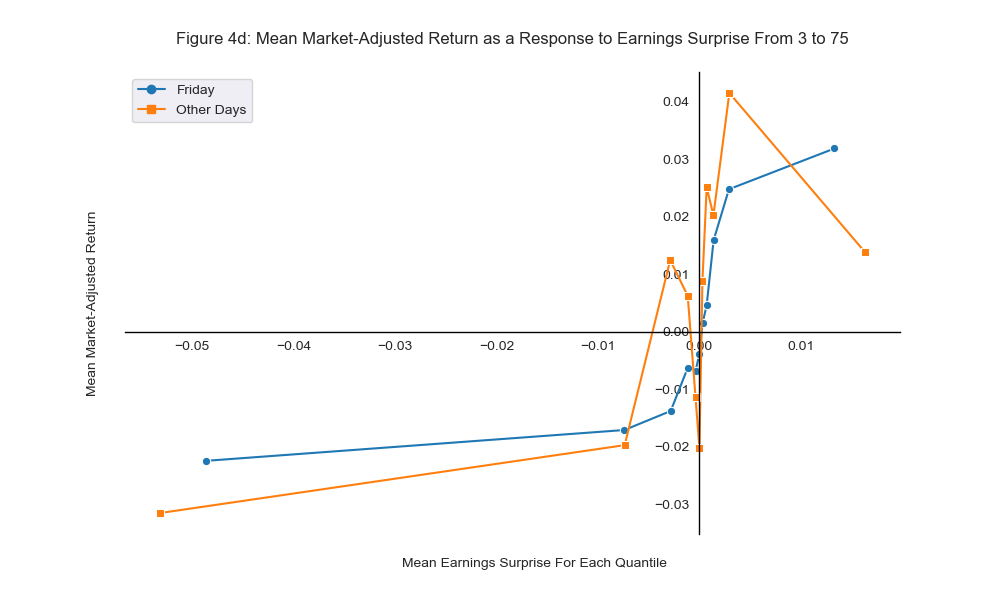
\includegraphics[width=.8\textwidth]{fig4d.png}
\end{figure}

\end{document}
